\documentclass[12pt,a4paper]{article}%
\usepackage{CJKutf8}
\usepackage{makeidx}
\makeindex
\usepackage{bm}
\usepackage{framed} % Easier way to use Framebox
\usepackage{pdfpages} % Import PDF in latex document
\usepackage{listings}
\usepackage{slashbox}
\usepackage{array}
\usepackage{enumitem}
\usepackage{amsmath, amssymb, amsthm}  % For mathematical symbols
\usepackage{colortbl,color}
\usepackage{xcolor}
\usepackage{auto-pst-pdf}
\usepackage{graphicx,psfrag}
\usepackage{tabularx,array}
\usepackage{booktabs}
\usepackage{multirow}
\usepackage{multicol}
\usepackage[subfigure]{tocloft}
\usepackage[tight]{subfigure}
\usepackage{float,booktabs,threeparttable}
\usepackage{caption}


\usepackage{longtable}
\usepackage{appendix}

\usepackage{pdfpages}
\usepackage{blkarray} %For adding Matrix label on row and column
\usepackage{url}
\usepackage{indentfirst} % indent the first paragraph of new section
\usepackage{titlesec} % change the way \subsubsubsection formats

\def\se{{\rm se}}
%\newcommand{\red}{\color{red}}
\linespread{1.5}  % The linespread is 1.5.

% Numbered theorems, definitions, algorithm and lemmas ======================================================================
\newtheorem{thm}{Theorem}  % Define new theorem.
\newtheorem{alg}{Algorithm}[section]  % Define new algorithm.
\newtheorem{definition}{Definition}
% ===========================================================================================================================

% For writing pseudo code ======================================================================
\usepackage{algorithm}% http://ctan.org/pkg/algorithms
\usepackage{algpseudocode}% http://ctan.org/pkg/algorithmicx
% ===========================================================================================================================

\theoremstyle{definition}
\theoremstyle{plain}
\setcounter{secnumdepth}{5}


\renewcommand{\contentsname}{Table of Contents}
\renewcommand{\listfigurename}{List of Figures}
\renewcommand{\listtablename}{List of Tables}
\renewcommand{\figurename}{\footnotesize Figure}
\renewcommand{\tablename}{\footnotesize Table}
\newcommand{\loflabel}{Figure}
\newcommand{\lotlabel}{Table}
\setlength{\abovecaptionskip}{0pt}


\renewcommand{\cftsecnumwidth}{7em}
\renewcommand{\appendixpagename}{\Large Appendix} % \ctxfb
\renewcommand{\arraystretch}{1.2}

\usepackage{appendix}



%%%%%%%%%%%%

\newtheorem{lma}{\textbf{Lemma}}

% ======================== Set length ========================
\setlength{\columnsep}{1cm}
\setlength\parindent{0pt}
\textheight = 22cm
\textwidth = 16.5cm
\hoffset=-1cm
\footskip=40pt
\renewcommand*{\arraystretch}{0.8}
% ============================================================
% ======================== Paragraph Indent ========================
\setlength{\parindent}{1em}
\setlength{\parskip}{1em}
% ==================================================================
% =============================
% Equation numbering
\numberwithin{equation}{section}
% =============================
% ======================== SubSubSubSection Format ========================
\titleclass{\subsubsubsection}{straight}[\subsection]

\newcounter{subsubsubsection}[subsubsection]
\renewcommand\thesubsubsubsection{\thesubsubsection.\arabic{subsubsubsection}}

\titleformat{\subsubsubsection}
  {\normalfont\normalsize\bfseries}{\thesubsubsubsection}{1em}{}
\titlespacing*{\subsubsubsection}
{0pt}{3.25ex plus 1ex minus .2ex}{1.5ex plus .2ex}
% ==================================================================


\begin{document}
\setcounter{section}{4}
\section{Resampling Methods}

\begin{itemize}
\item Goal
	\begin{enumerate}
	\item To choose the model with the most suitable flexibility level (model selection).
	\item The uncertainty (Standard error) in the parameter estimate can be measured by computing the sampling distribution of the estimator.
	\end{enumerate}
\end{itemize}

\subsection{\textbf{Cross-Validation}}
\subsubsection{\textbf{The Validation Set Approach}}
\begin{itemize}
\item \textbf{Implementation}:
	\begin{enumerate}
	\item Randomly divide observations in half, so $n/2$ as validation set and the other half as training set
	\item Compute the MSE for the validation set
	\item Repeat the steps stated above so we can get the results as Figure~\ref{figure-5.2}
	\end{enumerate}
\end{itemize}

\begin{figure}[H]
\centering
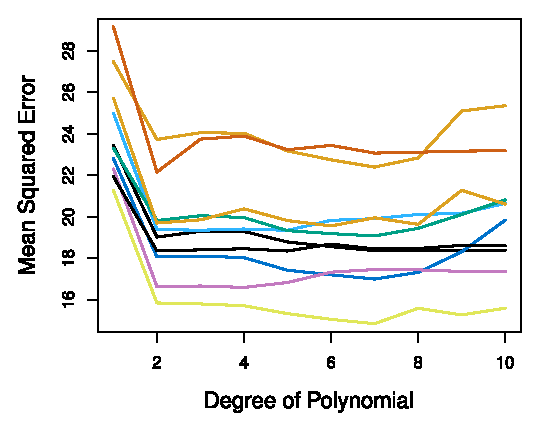
\includegraphics[scale=1]{images//5_2.eps}
\\~\\
\caption{}\label{figure-5.2}
\end{figure}

\begin{itemize}
\item Advantages
	\begin{enumerate}
	\item Before, we only choose part of the data as training set. Now, we should train our models on different set of data to overcome overfitting.
	\item From Figure~\ref{figure-5.2} we observed 10 curves indicate that the model with a quadratic term has a smaller validation set MSE then the model with only a linear term.
	      This helps us to choose the degree of polynomial when training a model.
	\end{enumerate}
\end{itemize}

\begin{itemize}
\item Drawbacks
	\begin{enumerate}
	\item The validation estimate of the test error can be highly variable, depending on which observations are included in the training set and in the validation set.
	\item In the validation approach only half of the data are used to fit the model. Since statistical methods tend to perform worse when trained on fewer observations. 
		  This implies the validation set error rate may tend to overestimate the test error rate for the model fit on the entire data set.
	\end{enumerate}
\end{itemize}

\subsubsection{\textbf{Leave-One-Out Cross-Validation (LOOCV)}}
\textbf{Implementation}:
\begin{table}[H]
\centering
\begin{tabular}{c | c | l}
Validation Set & Training Set & MSE \\
\hline 
$(x_{1},y_{1})$ & $\{(x_{2},y_{2}), (x_{3},y_{3}), \dots, (x_{n},y_{n}) \}$ & $\text{MSE}_{1}=(y_{1}-\hat{y}_{1})^{2}$ \\
\hline
$(x_{2},y_{2})$ & $\{(x_{1},y_{1}), (x_{3},y_{3}), \dots, (x_{n},y_{n}) \}$ & $\text{MSE}_{2}=(y_{2}-\hat{y}_{2})^{2}$  \\
\hline
$(x_{3},y_{3})$ & $\{(x_{1},y_{1}), (x_{2},y_{2}), \dots, (x_{n},y_{n}) \}$ & $\text{MSE}_{3}=(y_{3}-\hat{y}_{3})^{2}$  \\

$\vdots$ & $\vdots$ &  \multicolumn{1}{c}{$\vdots$}  \\

$(x_{n},y_{n})$ & $\{(x_{1},y_{1}), (x_{2},y_{2}), \dots, (x_{n-1},y_{n-1}) \}$ & $\text{MSE}_{n}=(y_{n}-\hat{y}_{n})^{2}$  \\
\hline
 & & $\text{CV}_{(n)}=\frac{1}{n}\sum\limits_{i=1}^{n} \text{MSE}_{i}$ \\
\hline
\end{tabular}
\end{table}

\begin{itemize}
\item Advantages
	\begin{enumerate}
	\item LOOCV create less bias. Since we repeatedly fit the method using training sets that contain $n-1$ observations.
	\item LOOCV does not overestimate the test error rate as much as the validation set approach does. 
	\item LOOCV will always yield the same results compared to validation set approach.
	\end{enumerate}
\end{itemize}

\begin{itemize}
\item Drawbacks
	\begin{enumerate}
	\item Computational expensive
	\end{enumerate}
\end{itemize}

\begin{figure}[H]
\centering
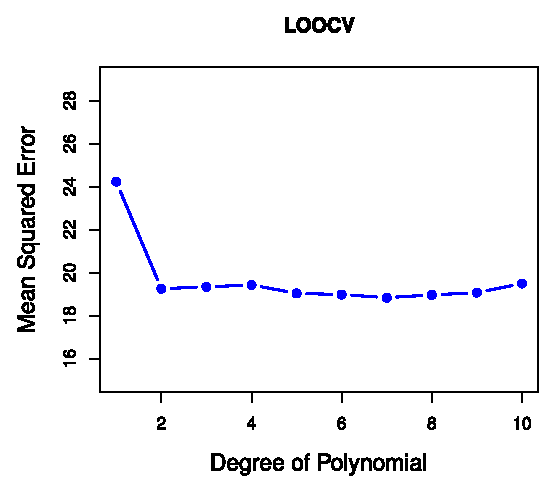
\includegraphics[scale=1]{images//5_4.eps}
\\~\\
\caption{The LOOCV error curve}\label{figure-5.4}
\end{figure}

\subsubsection{\textbf{k-Fold Cross-Validation}}
\begin{figure}[H]
\centering
\psfrag{A}[c][c]{Validation}
\psfrag{B}[c][c]{Training}
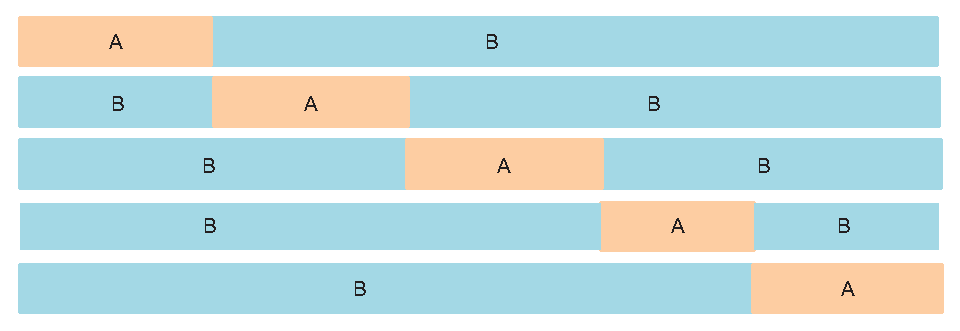
\includegraphics[scale=1]{images//5_5.eps}
\\~\\
\caption{5-fold CV. A set of $n$ observations is randomly split into five non-overlapping groups. If we set $k = n$, then we get LOOCV.}\label{figure-5.5}
\end{figure}

\begin{itemize}
\item \textbf{Implementation}:
	\begin{enumerate}
	\item $k=(1,\dots,n/k)$
	\item Randomly divide the data into $k$ groups, each group contains $n/k$ observations.
	\item Choose the $k$th fold as validation set, the other observations as training set.
	\item Compute the MSE for the $k$th fold.
	\item Repeat the process for $k$ times. 
	\end{enumerate}
\end{itemize}

\begin{equation*}
\text{CV}_{(k)}=\frac{1}{k}\sum\limits_{i=1}^{k} \text{MSE}_{i}
\end{equation*}
~\\
When we perform cross-validation, our goal might be to determine how well a method can be expected to perform on independent data; in this case, the actual estimate of the test MSE is of interest.
But at other times we are interested in finding the right flexibility level that fit the real data.
That means, we are looking for the flexibility level location of the minimum point in the estimated test MSE curve.

\begin{figure}[H]
\centering
\psfrag{A}[c][c]{Validation}
\psfrag{B}[c][c]{Training}
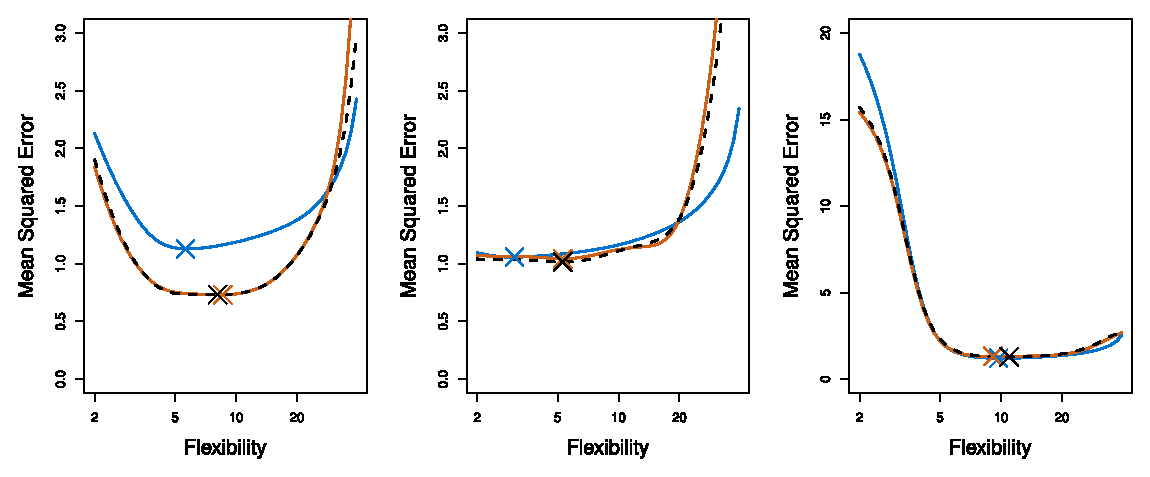
\includegraphics[scale=0.8]{images//5_6.eps}
\\~\\
\caption{All of the curves come close to identifying the correct levels of flexibility (the flexibility level corresponding to the smallest MSE)}\label{figure-5.6}
\end{figure}

\subsubsection{\textbf{Bias-Variance Trade-Off for k-Fold Cross-Validation}}
\begin{itemize}
\item \textbf{LOOCV}:
	\begin{itemize}
	\item Bias: approximately unbiased estimates of the test error, since each training set contains $n-1$ observations.
	\item Variance: higher variance, the MSE is averaging the outputs of $n$ fitted models and each iteration we are training on an almost identical set of observations; therefore, these outputs are highly correlated with each other.
	\end{itemize}
\end{itemize}

\begin{itemize}
\item \textbf{k-Fold CV}:
	\begin{itemize}
	\item Bias: intermediate level of bias, since each training set contains $n-\frac{n}{k}$ observations
	\item Variance: lower variance, the MSE is the averaging the outputs of $k$ fitted model (less fitted model than LOOCV) that are less correlated with each other, since the overlap between the training sets in each model is smaller.
	\end{itemize}
\end{itemize}

\subsubsection{\textbf{Cross-Validation on Classification Problems}}

\begin{equation*}
\text{CV}_{(n)} = \frac{1}{n}\sum\limits_{i=1}^{n} I(y_{i} \neq \hat{y}_{i})
\end{equation*}

\begin{figure}[H]
\centering
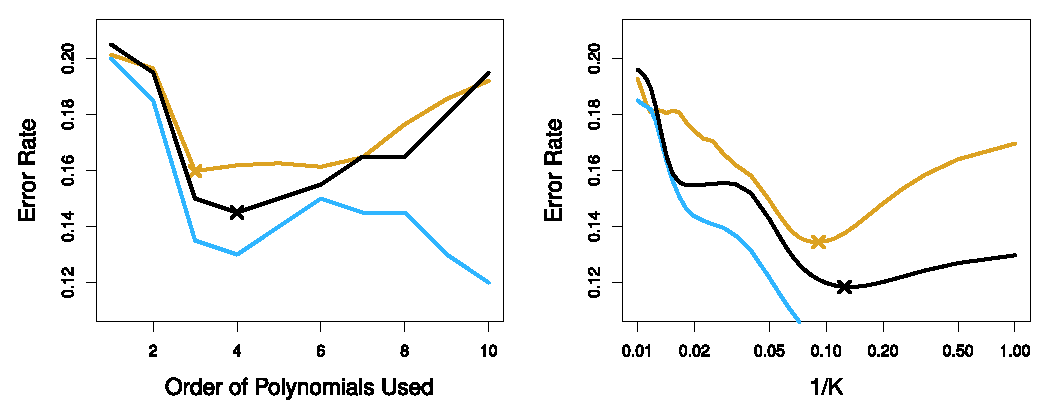
\includegraphics[scale=1]{images//5_8.eps}
\\~\\
\caption{Test error(brown), training error(blue) and 10-fold CV error(black) Left: Logistic Regression using polynomial functions of the predictore. Right: The KNN classifier with different values of $K$}\label{figure-5.8}
\end{figure}

From Figure~\ref{figure-5.8} we find that the test error displays a characteristic of U-shape. The 10-fold CV error rate provides a good approximation to the test error rate. 
The 10-fold CV reaches a minimum when fourth-order polynomials are used, which is very close to the minimum of the test error curve, which occurs when third-order polynomials are used. 


\subsection{\textbf{The Bootstrap}}
Bootstrap is a simple Monte Carlo technique to approximate the sampling distribution. 
Through the sampling distribution, we can evaluate how good our data fit to the model.

Suppose we have a model fit to a set of training data. We denote the training set by $\boldsymbol{Z} = (z_{1},z_{1},\dots,z_{N})$ where $z_{i}=(x_{i},y_{i})$.  

\begin{itemize}
\item \textbf{Implementation}:
	\begin{enumerate}
	\item Randomly draw data sets with replacement from the training data. Each sets $\boldsymbol{Z}^{*b}$ contains $N$ observations.
	\item By plugging the data sets $\boldsymbol{Z}^{*b}$ to the estimator $S(\cdot)$ we defined, we get our estimates $S(\boldsymbol{Z}^{*b})$. 
	\item We can estimate any aspect of the distribution of $S(\boldsymbol{Z})$, say, its variance, $\widehat{\text{Var}}[S(\boldsymbol{Z})].$ where $\bar{S}^{*} = \sum_{b} S(\boldsymbol{Z}^{*b})/B$
	\end{enumerate}
\end{itemize}

One approach to estimate prediction error is to fit the model on a set of bootstrap samples, and then keep track of how well it predicts the original training set. 
If $\hat{f}^{*b}(x_{i})$ is the predicted value at $x_{i}$, from the model fitted to the $b$th bootstrap dataset, our estimate is 

\begin{equation*}
\widehat{\text{Err}_{\text{boot}}} = \frac{1}{B} \frac{1}{N} \sum\limits_{b=1}^{B} \sum\limits_{i=1}^{N} (y_{i}-\hat{f}^{*b}(x_{i}))^{2}
\end{equation*}

The bootstrap implementation can be illustrated as below Figure,
\begin{framed}
\begin{figure}[H]
\centering
\psfrag{a}[c][c]{Training Set}
\psfrag{b}[c][c]{Bootstrap Samples}
\psfrag{c}[c][c]{Prediction Error}
\psfrag{A}[r][l]{\parbox{1cm} {$\boldsymbol{Z}=(z_{1},z_{2},\dots,z_{N})$}}
\psfrag{B}[l][l]{\footnotesize \parbox{1cm}{  
\begin{gather*}
\boldsymbol{Z}^{*1} = 
\begin{array}{c}
(x^{*1}_{1},y^{*1}_{1}) \\
(x^{*1}_{2},y^{*1}_{2}) \\
\vdots \\
(x^{*1}_{N},y^{*1}_{N})
\end{array}
\end{gather*}
}}
\psfrag{C}[l][l]{\footnotesize \parbox{1cm}{  
\begin{gather*}
\boldsymbol{Z}^{*2} = 
\begin{array}{c}
(x^{*2}_{1},y^{*2}_{1}) \\
(x^{*2}_{2},y^{*2}_{2}) \\
\vdots \\
(x^{*2}_{N},y^{*2}_{N})
\end{array}
\end{gather*}
}}
\psfrag{D}[l][l]{\footnotesize \parbox{1cm}{  
\begin{gather*}
\boldsymbol{Z}^{*B} = 
\begin{array}{c}
(x^{*B}_{1},y^{*B}_{1}) \\
(x^{*B}_{2},y^{*B}_{2}) \\
\vdots \\
(x^{*B}_{N},y^{*B}_{N})
\end{array}
\end{gather*}
}}
\psfrag{E}[l][l]{\hspace{0.5cm} \footnotesize $\boldsymbol{Z}^{*1} \sim \hat{f}^{*1}$}
\psfrag{F}[l][l]{\hspace{0.5cm} \footnotesize $\boldsymbol{Z}^{*2} \sim \hat{f}^{*2}$}
\psfrag{G}[l][l]{\hspace{0.5cm} \footnotesize $\boldsymbol{Z}^{*B} \sim \hat{f}^{*B}$}

\psfrag{H}[c][c]{\footnotesize $\sum\limits_{i=1}^{N}(y_{i}-\hat{f}^{*1}(x_{i}))^{2}$}
\psfrag{I}[c][c]{\footnotesize $\sum\limits_{i=1}^{N}(y_{i}-\hat{f}^{*2}(x_{i}))^{2}$}
\psfrag{J}[c][c]{\footnotesize $\sum\limits_{i=1}^{N}(y_{i}-\hat{f}^{*B}(x_{i}))^{2}$}
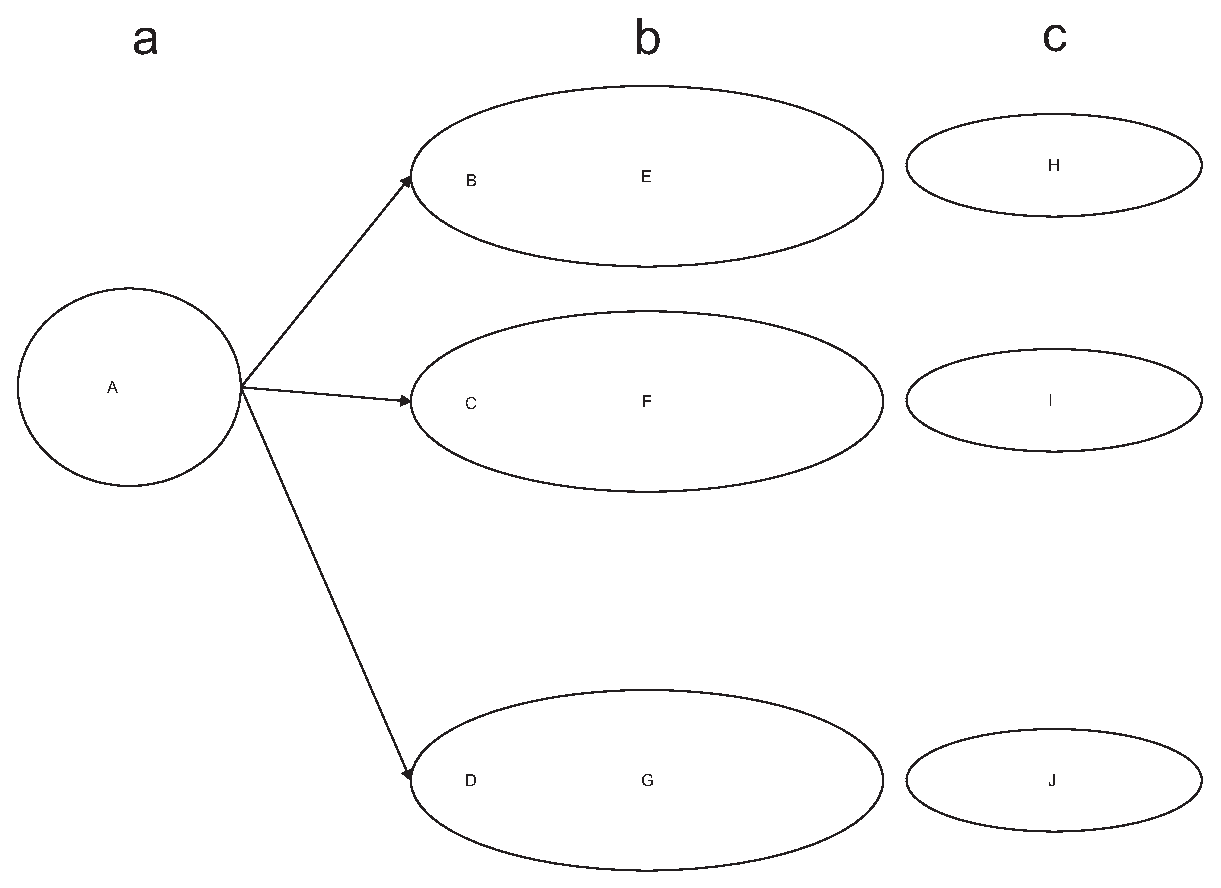
\includegraphics[scale=0.8]{images//bootstrap.eps}
\\~\\
\caption{}\label{bootstrap}
\end{figure}
\end{framed}

However, $\widehat{\text{Err}_{\text{boot}}}$ is not a good way of estimating prediction error. 
The reason is that the bootstrap datasets are acting as the training samples, while the original traiing set is acting as the test sample, and these two samples have observations in common. 
This overlap can make overfit predictions look unrealistically good. \\

In order to solve this issue, we apply the leave-one-out bootstrap estimate of prediction error, this is, 
\begin{equation*}
\widehat{\text{Err}}^{(1)} = \frac{1}{N} \sum\limits_{i=1}^{N} \frac{1}{|C^{-i}|} \sum\limits_{b \in C^{-i}} (y_{i}-\hat{f}^{*b}(x_{i}))^{2} 
\end{equation*}

\begin{itemize}
\item $C^{-i}$ : The set of indices of the bootstrap samples $b$ that do not contain observation $i$ 
\item $|C^{-i}|$ : the number of such bootstrap samples
\end{itemize}


\begin{figure}[H]
\centering
\psfrag{A}[r][l]{\footnotesize $z_{1}=(x_{1},y_{1})$}
\psfrag{B}[c][c]{\footnotesize $z_{1} \not\in \boldsymbol{Z}^{*1} $}
\psfrag{C}[c][c]{\footnotesize $z_{1} \not\in \boldsymbol{Z}^{*2}$}
\psfrag{D}[c][c]{\footnotesize $z_{1} \in \boldsymbol{Z}^{*3}$}
\psfrag{E}[c][c]{\footnotesize $(y_{1}-\hat{f}^{*1}(x_{1}))^{2}$}
\psfrag{F}[c][c]{\footnotesize $(y_{1}-\hat{f}^{*2}(x_{1}))^{2}$}
\psfrag{G}[c][c]{\footnotesize null}
\psfrag{H}[c][c]{\footnotesize $\frac{1}{2} \sum\limits_{b=1}^{2} (y_{1}-\hat{f}^{*b}(x_{1}))^{2}$}
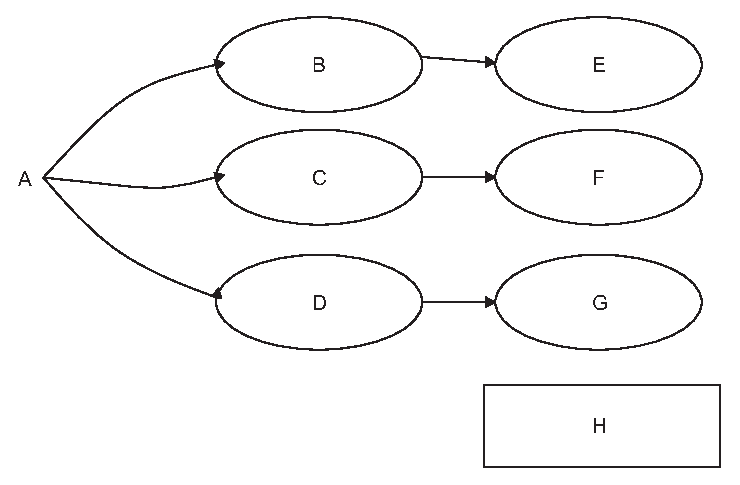
\includegraphics[scale=0.8]{images//bootstrap_loo.eps}
\\~\\
\caption{The figure gives an example on $z_{1}=(x_{1},y_{1})$. After repeating the process through all the observations ($z_{2},\dots,z_{N}$) and summarize them, we can get $\widehat{\text{Err}}^{(1)}$.}\label{bootstrap_loo}
\end{figure}

The ".632 estimator" is designed to alleviate this bias. It is defined by,
\begin{equation*}
\widehat{Err}^{(.632)} = .368 \cdot \overline{\text{err}} + .632 \cdot \widehat{\text{Err}}^{(1)}
\end{equation*}

$\overline{\text{err}}$ is the training error. The derivation of the .632 estimator is complex; intuitively it pulls the leave-one out bootstrap estimate($\widehat{\text{Err}}^{(1)}$) down toward the training error rate, and hence reduces its upward bias.


\subsection{Exercises}
%====================================================================================================================================
% 2.====================================================================================================================================
\begin{enumerate}
\item[2.] We will now derive the probability that a given observation is part of a bootstrap sample. Suppose that we obtain a bootstrap sample from a set of $n$ observations.
\begin{enumerate}
	\item[(a)] What is the probability that the first bootstrap observation is not the $j$th observation from the original sample? Justify your answer.
	\item[(b)] What is the probability that the second bootstrap observation is not the $j$th observation from the original sample?
	\item[(c)] Argue that the probability that the $j$th observation is not in the bootstrap sample is $(1-1/n)^{n}$.
	\item[(d)] When $n = 5$, what is the probability that the $j$th observation is in the bootstrap sample?
	\item[(e)] When $n = 100$, what is the probability that the $j$th observation is in the bootstrap sample?
	\item[(f)] When $n = 10000$, what is the probability that the $j$th observation is in the bootstrap sample?
	\item[(g)] Create a plot that displays, for each integer value of $n$ from 1 to 100000, the probability that the $j$th observation is in the bootstrap sample. Comment on what you observe.
	\item[(h)] We will now investigate numerically the probability that a bootstrap sample of size $n = 100$ contains the $j$th observation. Here $j = 4$. We repeatedly create bootstrap samples, and each time we record whether or not the fourth observation is contained in the bootstrap sample.
\end{enumerate}
\end{enumerate}


\begin{oframed}
Answer: ~\\
$A$ : The event that the bootstrap observation is the $j$th observation from the original data set. \\
$A'$ : The event that the bootstrap observation is not the $j$th observation from the original data set. \\
$P(A)$ : The probability that the bootstrap observation is the $j$th observation from the original data set. \\
$P(A')= 1-P(A)$ : The probability that the bootstrap observation is not the $j$th observation from the original data set.
\begin{enumerate}
	\item[(a)] $P(A') = 1-\frac{1}{n}$
	\item[(b)] $P(A') = 1-\frac{1}{n}$
	\item[(c)] We draw $n$ times from the original sample with replacement, so the probability that for $n$ repeat drawings, the $j$th observation is not include in the bootstrap is,
		\begin{equation*}
			P(A')^{n} = (1-\frac{1}{n})^{n}
		\end{equation*}
	\item[(d)] Probability of the $j$th obs. in 5 observations bootstrap sample : \\ $ 1-P(A')^{5} = 1-(1-\frac{1}{5})^{5} = 0.67232$
	\item[(e)] Probability of the $j$th obs. in 100 observations bootstrap sample : \\ $ 1-P(A')^{100} = 1-(1-\frac{1}{100})^{100} = 0.63397 $	
	\item[(f)] Probability of the $j$th obs. in 10000 observations bootstrap sample: \\ $ 1-P(A')^{10000} = 1-(1-\frac{1}{10000})^{10000} = 0.6321  $	
	\item[(g)] $P(\text{observation }i \in \text{bootstrap sample } b) = 1-(1-\frac{1}{n})^{n} = 1-e^{-1}=0.632$. \\
			   This implies the average number of distinct observations in each bootstrap sample is about $0.632 \cdot n$, so its bias will roughly behave like that of twofold cross-validation.
			   More detail in The Elements of Statistical Learning Section 7.11.
\end{enumerate}
\end{oframed}

\begin{CJK}{UTF8}{cwmb}
\section*{Reference}
\noindent
\begin{description}\itemsep=-2pt
\item 張翔 (2012), 《提綱契領學統計》, 四版, 鼎茂圖書
\item Friedman, J., Hastie, T., \& Tibshirani, R. (2001). {\it{The elements of statistical learning}} (Vol. 1). Springer, Berlin: Springer series in statistics.
\item James, G., Witten, D., Hastie, T., \& Tibshirani, R. (2013). {\it{An introduction to statistical learning}} (Vol. 6). New York: springer.
\item Wasserman, L. (2013). {\it{All of statistics: a concise course in statistical inference}}. Springer Science \& Business Media.
\item J Li, Linear Discriminant Analysis, \url{http://sites.stat.psu.edu/~jiali/course/stat597e/notes2/lda.pdf}
\end{description}
\end{CJK}

\end{document}
